\documentclass[12pt]{article}
\usepackage{verbatim}
\usepackage[dvips]{epsfig}
\usepackage{color}
\usepackage{url}
\usepackage[colorlinks=true]{hyperref}

\begin{document}

\section*{GENESIS: Documentation}

{\bf Related Documentation:}
% start: userdocs-tag-replace-items related-do-nothing
% end: userdocs-tag-replace-items related-do-nothing

\section*{Functional User Specification for the G-Tube}
This functional user specification for the GENESIS GUI ({\bf G-Tube}) is based on the four steps of the Publication Workflow (see Fig. \ref{fig:wf-pub-1}). This specification covers single cell models.

\begin{figure}[h]
  \centering
   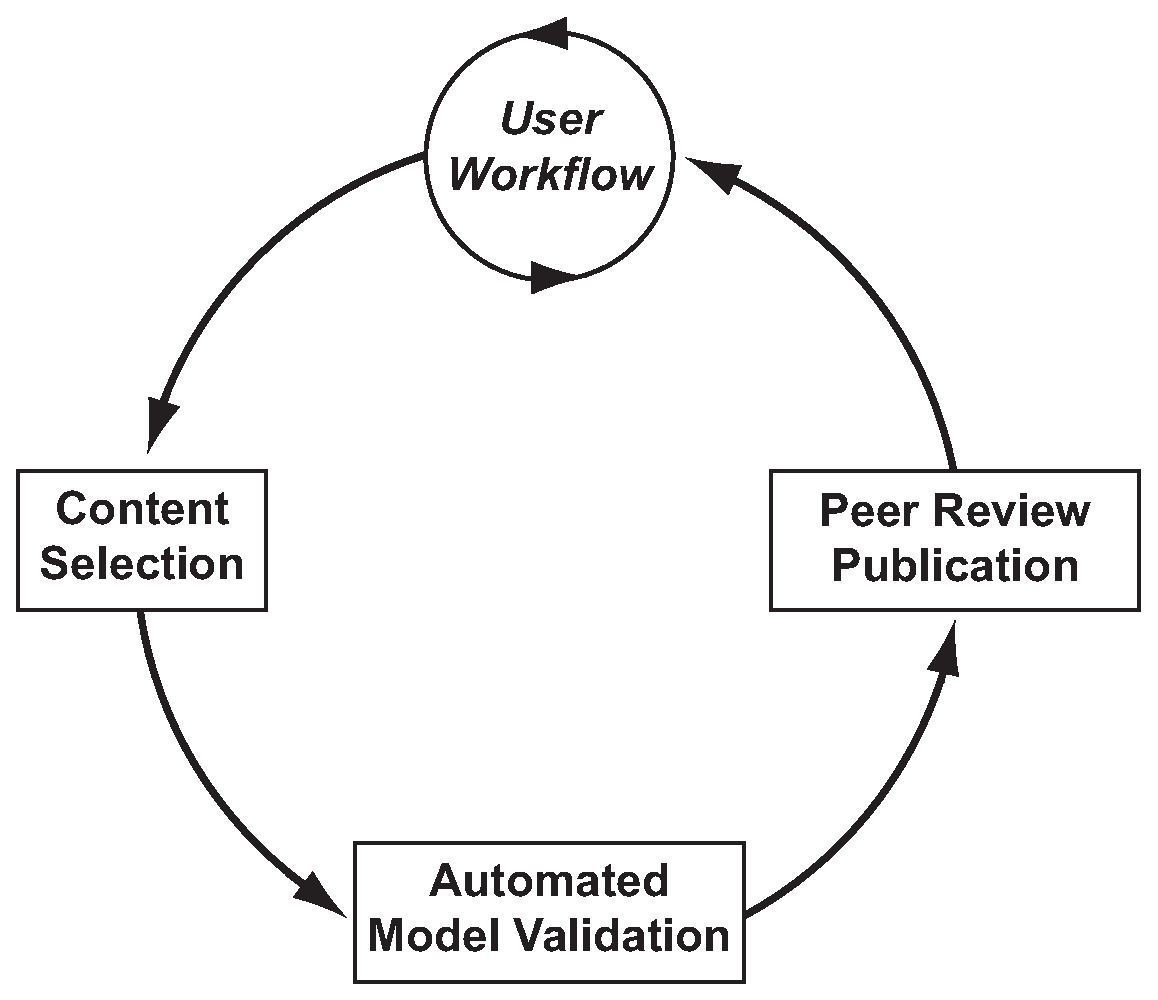
\includegraphics[scale=0.3]{figures/g3-publication-workflow-circular.eps}
\caption{{\bf Publication Workflow:} The four steps of the Publication Workflow. The first step of the Publication Workflow is provided by the User Workflow (see Fig. \ref{fig:wf-user-1}).}
  \label{fig:wf-pub-1}
\end{figure}

\begin{figure}[h]
  \centering
   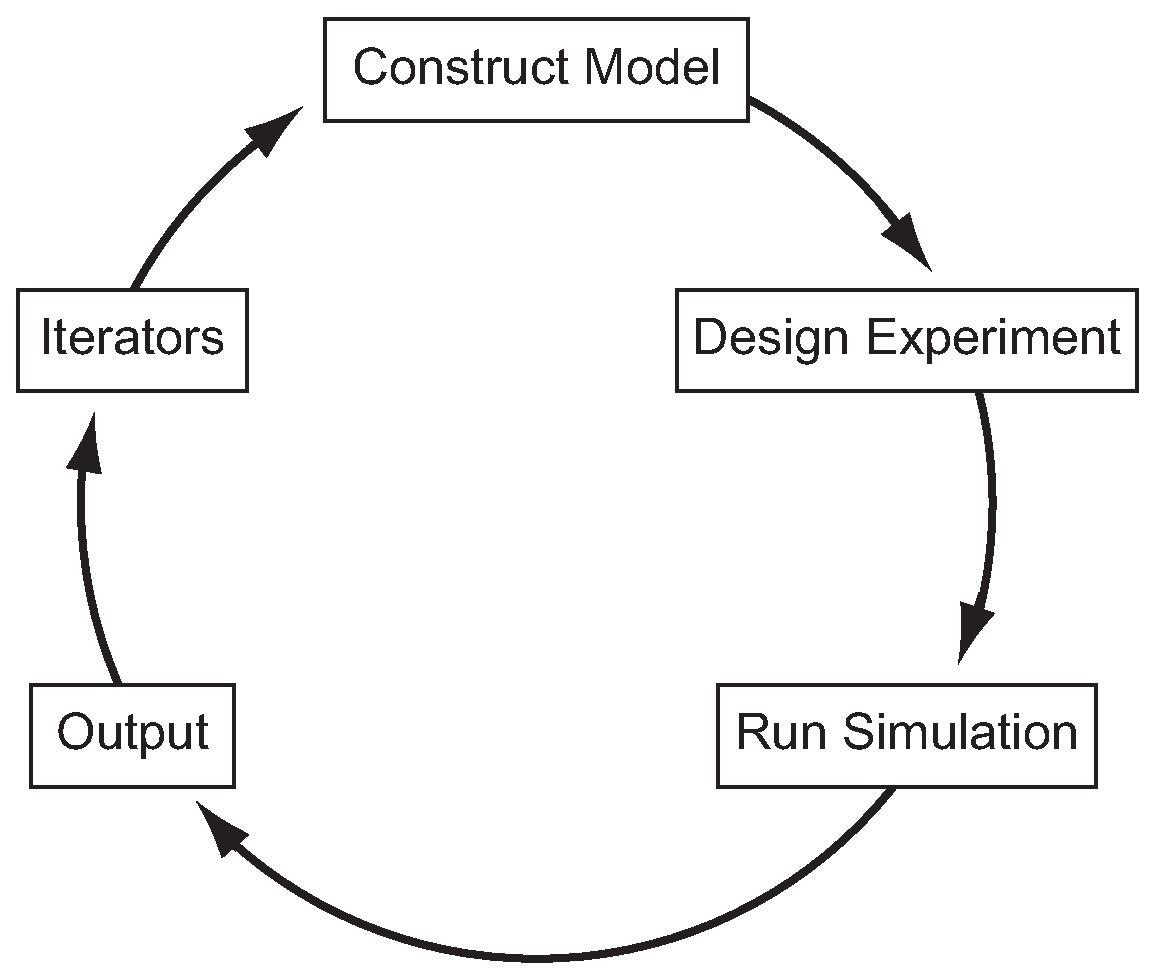
\includegraphics[scale=0.25]{figures/g3-user-workflow-circular.eps}
\caption{{\bf User Workflow:} The five steps of the User Workflow. The completed User Workflow is embedded in the first step in the Publication Workflow (see Fig. \ref{fig:wf-pub-1}).}
  \label{fig:wf-user-1}
\end{figure}

\begin{figure}[h]
  \centering
   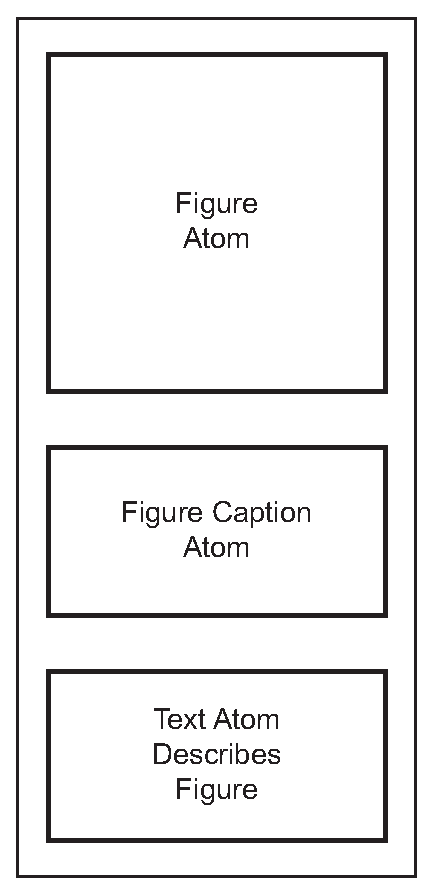
\includegraphics[scale=0.5]{figures/g3-publication-molecule.eps}
\caption{{\bf Figure Molecule:} Example relationship between publication atoms and a (figure) molecule.}
  \label{fig:pm-1}
\end{figure}

\begin{figure}[h]
  \centering
   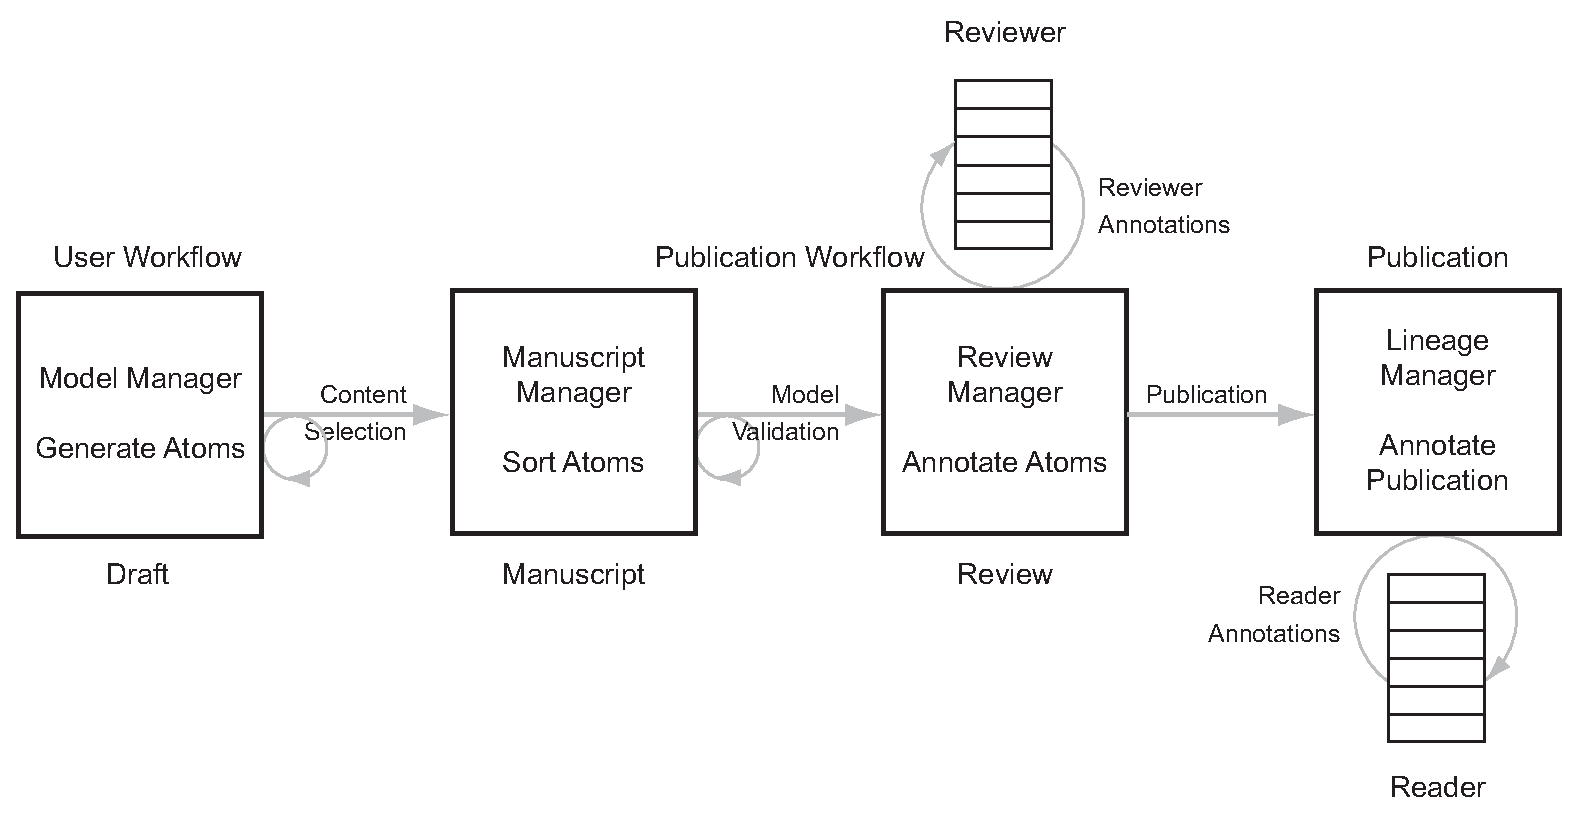
\includegraphics[scale=0.5]{figures/g3-atom-pipeline.eps}
\caption{{\bf Atom Pipeline:} Technical specification of relationship between publication atoms and the Publication Workflow.}
  \label{fig:ap-1}
\end{figure}

\begin{enumerate}
   \item{\bf User Workflow:}\\Selecting the ``User Workflow'' tab presents the User Workflow panel that contains the following selectable menu items.

     \begin{enumerate}
     
      \item{\bf Construct Model:}
         \begin{enumerate}
            \item{\bf Import Model:}\\Load and open a pre-existing project environment in the GUI. Default: NDF format. Other loadable file formats include: NeuroML, 9ML, or from a GENESIS 2 model imported via the {\bf NS-SLI} module.
            \item{\bf Create Model:}
               \begin{enumerate}
                  \item{\bf Create single compartment model:}
                     \begin{itemize}
                        \item Create compartment.
                        \item Define passive membrane parameters.
                     \end{itemize}
                     
                  \item{\bf Create multi-compartment model:}
                     \begin{itemize}
                        \item Import cell morphology.
                        \item Define passive membrane parameters for soma and dendrites. Default: Somatic and dendritic parameters identical.
                     \end{itemize}
                     
                     \item{\bf Populate model:}
                        \begin{itemize}
                           \item Add channel types from channel model library.
                           \item Define $\bar g$ for each channel type.
                           \item Define 1-D distribution of channel densities for each channel type included in multicompartment model. Choice of:
                              \begin{itemize}
                                 \item {\bf Uniform:} Default for dendrites and soma. Can be set independently for soma and dendrites.
                                 \item {\bf Gamma:} Dendritic density defined by absolute ortho- or antidromic distance from soma along single dendrites.
                              \end{itemize}
                        \end{itemize}
                \end{enumerate}
                
           \item{\bf Modify model parameter values:}
                       
            \item{\bf Model summary:}\\Generate tables containing passive membrane properties and channel, synaptic, and gap-junction parameter values (if present).
            \item{\bf Save tables:}  Generated during model checking step of User Workflow.
               \begin{itemize}
                  \item{\bf Black:} Default values.
                  \item {\bf Green:} User modified values.
                  \item{\bf Red:} Problematic values, e.g. out of expected range.
               \end{itemize}
            \item {\bf Annotate tables:}

            \item{\bf Explore model:}
                  \begin{enumerate}
                     \item {\bf Generate list of model compartments:} Selecting one or more compartments from this list generates a list of properties, components, and parameter values for each selected compartment.
                     \item {\bf Selected compartments:} Map to 3-D scalable and rotatable cell morphology.
                     \item {\bf Generate list of model components:} Selecting a model component generates a list of compartments that contain the given component. Location of selected components map to 3-D scalable and rotatable cell morphology.
                  \end{enumerate}
                  
            \item{\bf Annotate model:}\\Record source of any changes made to published parameters (the default parameter values of the model). This should include whether the source is one of the following:
               \begin{itemize}
                  \item Citation for published source of new values.
                  \item Obtained from simulations.
               \end{itemize} 
            
            \item {\bf Save model:} Choice of NDF, NeuroML or 9ML file formats. Model can be saved in one or more formats. Default format: NDF.
         \end{enumerate}
         
      \item{\bf Design Experiment:}
         \begin{enumerate}
            \item{\bf Choose inputs:}
               \begin{enumerate}
                  \item{\bf Set stimulus type:} One of:
                     \begin{itemize}
                        \item Current injection.
                        \item Current clamp.
                        \item Voltage clamp.
                        \item Synaptic stimulation.
                     \end{itemize}
                     \item{\bf Set specific parameter values of stimulus protocol:}
                        \begin{itemize}
                           \item{\bf Current injection:} Set magnitude and duration.
                           \item{\bf Current clamp:} Set magnitude and duration.
                           \item{\bf Voltage clamp:} Set holding potential and duration.
                           \item{\bf Synaptic stimulation:}
                              \begin{itemize}
                                 \item Dendritic location.
                                 \item Number of synapses.
                                 \item Frequency.
                                 \item Temporal distribution of impulses: uniform, poisson, gamma.
                              \end{itemize}
                        \end{itemize}
                  \item{\bf Choose outputs:}
                     \begin{itemize}
                        \item Select and set parameter values to be saved.
                     \end{itemize}
                  \item{\bf Choose output resolution:}
                 \item{\bf Save experimental design:} Automatically saved as part of {\bf SSP} file.
              \end{enumerate}
         \end{enumerate}
         
      \item{\bf Run Simulation:}
         \begin{enumerate}
            \item{\bf Set and check runtime options:}
               \begin{itemize}
                  \item Update time step duration: fixed or variable.
                  \item Simulation duration.
                  \item Visualize runtime parameters.
               \end{itemize}
            \item{\bf Run simulation:}
            \item{\bf Save model state:} This can be used to eliminate time required for model startup.
            \item{\bf Reset simulation:} Set solver variables to values given by one of:
               \begin{itemize}
                  \item Default: Initial state of last model saved.
                  \item Specified previously saved model state.
               \end{itemize}
         \end{enumerate}
         
      \item{\bf Output:}
         \begin{enumerate}
            \item{\bf Construct draft atoms:} For example see Fig. \ref{fig:pm-1}.
            \begin{itemize}
               \item{\bf Internally:} Via {\it g3plot} and/or the {\bf Studio}.
               \item {\bf Externally:} Via Matlab, xmgrace, Mathematica, etc.
            \end{itemize}
            \item{\bf Import externally generated figures, graphs and tables:}
            \item{\bf Check simulation output:} Does expected output exist.
            \item{\bf Check validity of results:} Does output make sense.
            \item{\bf Analyze output:} Statistical analysis.
            \item{\bf Annotate draft atoms:}.
         \end{enumerate} 
              
      \item{\bf Iterators:}
        \begin{enumerate}
           \item{\bf Batch file construction:}
              \begin{itemize}
                 \item {\bf Manual:} From text editor generate {\bf SSP} file variants..
                 \item{\bf Automated:} Use scripts to automatically generate {\bf SSP} file variants.
              \end{itemize}   
           \item{\bf Dynamic Clamp:} RTXI.
           \item {\bf Note:} During completion of the User Workflow a numbered list is constructed of all ``Draft'' atoms (see Fig. \ref{fig:ap-1}).
         \item{\bf Select Draft Atoms for inclusion in Manuscript:} The components of a project to be included in a publication are selected from draft atoms generated during completion of the User-Workflow. In the content selection step (following), these atoms become "Manuscript" atoms.
        \end{enumerate}
      \end{enumerate}
            
   \item{\bf Content Selection:}
      \begin{enumerate}
         \item{\bf Gather selected manuscript atoms:}
          \item{\bf Organize selected manuscript atoms:} The list of atoms chosen by an investigator for publication can be ordered.
     \end{enumerate}

   \item{\bf Automated Model Validation:}\\Ensure lineage starting point of the model employed for simulations is a previously published source model.
      \begin{enumerate}
         \item{\bf Model verification:} Performed on
            \begin{itemize}
               \item Morphology.
               \item Cable discretization.
               \item Equations for different membrane and synaptic channel types and their kinetics.
               \item Model parameter values.
               \item Dynamic response to specific current injection and voltage clamp protocols.
            \end{itemize}
         \item{\bf Test robustness of parameter values:} Assess fragility of new or changed model parameters.
         \item{\bf Verify parameter values:} Determine `normality� of new or changed parameters used by model.
         \item{\bf Check publication atoms:} Numerical values cited in publication atoms are compared with model values.
         \item{\bf Verify figures:} Check all figures are generated by the same model.
         \item{\bf Identify changes to base model:} Compare project model to base model.
            \begin{itemize}
               \item Check morphology.
               \item Check parameter values.
            \end{itemize}
         \item{\bf Identify source of changed values:} Are changed values from new experimental data or simulations.
      \end{enumerate}

   \item{\bf Peer Review/Publication:}
      \begin{enumerate}
         \item{\bf Automated validation report:} Provides technical summary.
            \begin{itemize}
               \item Morphology.
               \item Parameters.
               \item Equations.
               \item Figures.
               \item Tables.
               \item References.
            \end{itemize}
         \item{\bf Human review:}
            \begin{itemize}
               \item Narrative.
               \item Model.
               \item Model extensions.
               \item Novelty.
               \item Significance.
            \end{itemize}
      \end{enumerate}

\end{enumerate}

%\bibliographystyle{plain}
%\bibliography{../tex/bib/g3-refs.bib}

\end{document}
